%---------------------------------------------------------------------------------
%                西南交通大学研究生学位论文：第一章内容
%---------------------------------------------------------------------------------
\chapter{绪论}

\section{研究背景与意义}

\subsection{研究背景}

数字政府建设正在持续推动政务数据资源沉淀，并使数据逐步成为政府治理的重要生产要素。
2022年，国务院印发《关于加强数字政府建设的指导意见》，明确提出以数据资源开发利用贯通政府管理、公共服务和科学决策各环节，充分释放数据要素价值\cite{guowuyuan2022digital}。
2023年，中共中央、国务院印发《数字中国建设整体布局规划》，进一步将数字政府和数据资源体系建设上升为国家战略部署\cite{zhonggong2023shuzichina}。
2025年，国家发展改革委、国家数据局、工业和信息化部联合印发《国家数据基础设施建设指引》，从数据流通利用、算力底座、网络支撑和安全防护等方面提出总体建设方向，强调以基础设施能力支撑数据高效流通与应用开发\cite{ndrc2025infrastructure}。
在上述政策持续推动下，各级政府部门不断推进数据归集、治理与共享交换，财政预算、公共资源、社会治理、经济运行等场景积累了大量结构化政务数据，政务数据已经成为支撑政府业务协同、治理监测和科学决策的重要基础\cite{孟天广2021,张聪丛2024}。

然而政务数据规模的快速增长并未自然转化为高效的数据使用能力。当前政务数据应用仍主要依赖两种模式：一是由技术人员编写SQL语句完成数据库查询，再由业务人员进行人工解读和汇总；二是通过预置报表和BI看板查看固定口径的统计结果。
前者对使用者的数据库知识、统计分析能力和业务理解能力要求较高，难以支撑非技术岗位开展自主问数；
后者虽然降低了操作门槛，但通常只能提供预定义维度下的静态展示，难以满足临时性、多维度和深层次的数据探索需求\cite{孟天广2021,张聪丛2024}。
与此同时，政务任务普遍具有跨部门、跨层级和跨区域协同特征，围绕协同治理形成的数据又呈现出显著的时空性、层级性和业务约束性。
已有研究表明，面向政府大规模协同任务的数据管理与统计分析本身就具有较高复杂度，传统离线处理和割裂式系统难以及时响应复杂场景下的动态分析需求\cite{王璐璐2023}。
这使得政务数据应用长期面临“数据可得但难用、报表可看但难析、需求可提但响应滞后”的现实困境。

\begin{figure}[htbp]
	\centering
	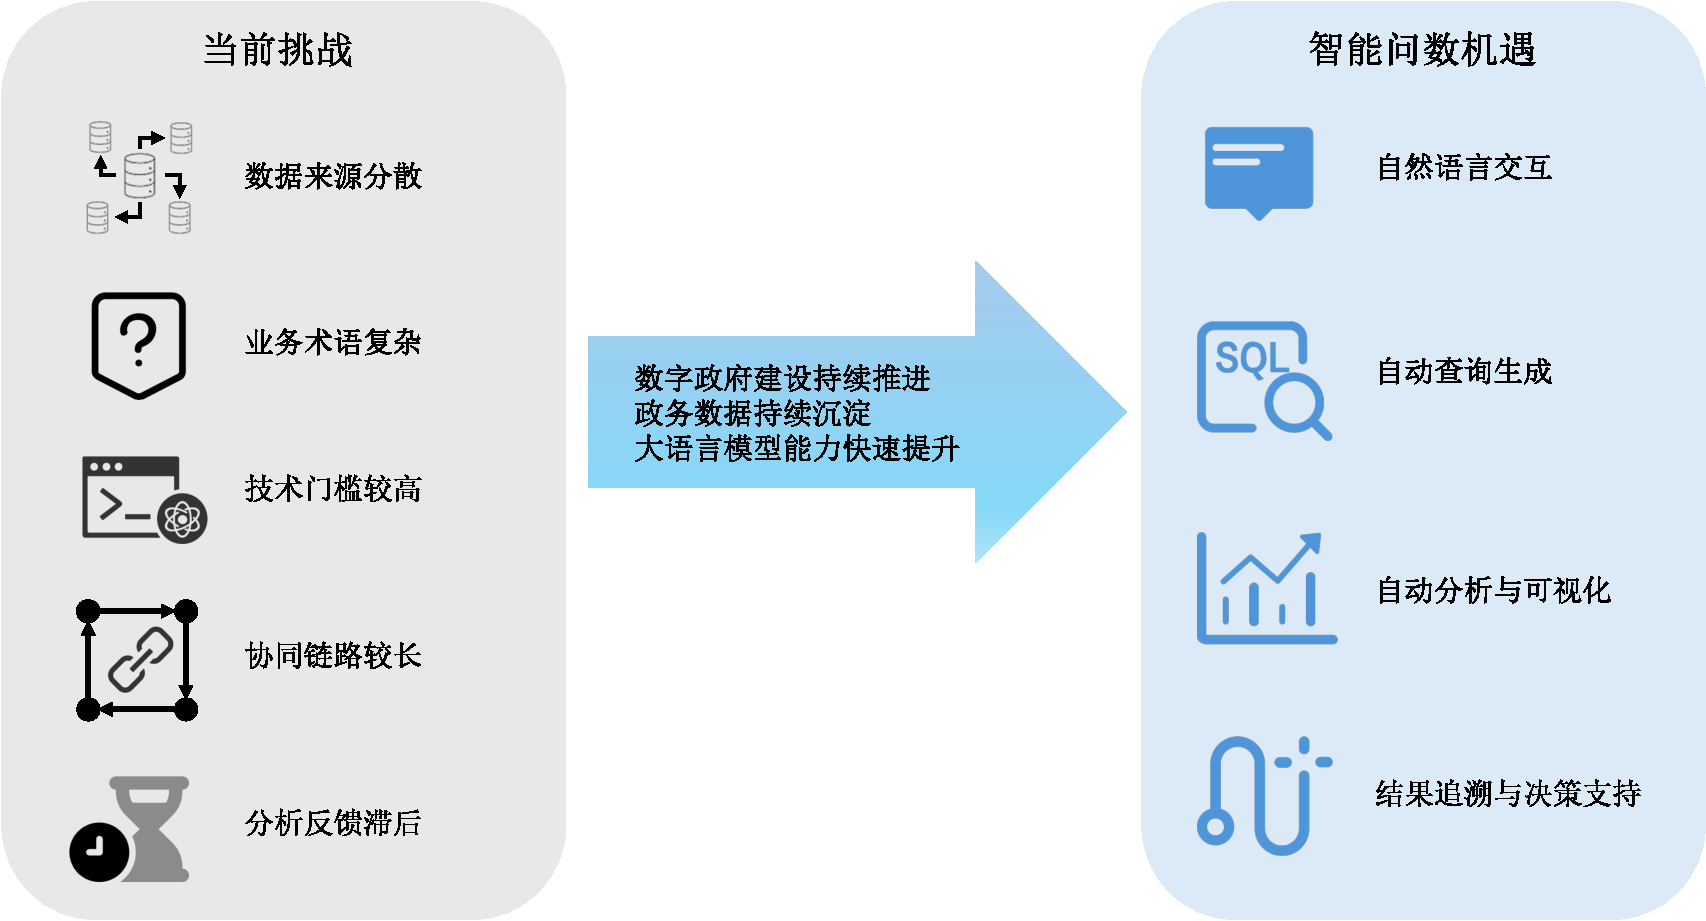
\includegraphics[width=0.9\textwidth]{figures/chap01/chap01-challenge.pdf}
	\caption{政务数据应用面临的挑战与智能问数带来的机遇示意图}
	\label{fig:chap01_challenge_opportunity}
\end{figure}

近年来以GPT-4\cite{openai2023gpt4}、Qwen\cite{qwen2024}和DeepSeek\cite{deepseek2024}为代表的大语言模型在自然语言理解、代码生成、复杂推理和工具调用等方面表现出显著能力提升\cite{zhao2023llmsurvey}，推动自然语言问数、自动代码生成和自动数据分析等方向快速发展。在数据查询层面，Text-to-SQL技术已能够将自然语言问题自动转换为结构化查询语句\cite{liu2025survey}；在数据分析层面，大语言模型结合代码执行和分析规划能力，开始具备围绕数据结果生成图表、表格和分析结论的潜力\cite{hong2024datainterpreter,gu2024analysts}。从国内应用看，大语言模型已逐步进入交通、民生服务和政务服务等垂直领域，基于自然语言交互的智能问数模式正从概念验证走向场景化探索\cite{王昀2024,沈宇2025,兰洪浩2025}。但政务场景中的数据语义、统计口径和结果规范性要求显著高于通用商业场景，直接迁移通用方法往往仍面临领域知识融入不足、分析流程缺乏结构化约束、查询与分析环节协同不畅等问题。

基于上述场景、瓶颈和技术现状，本文聚焦于政务领域智能问数与数据分析这一研究主题，关注的问题不是单一的“自然语言转SQL”，而是如何围绕政务业务语义构建一条从自然语言需求理解、可靠查询生成、规范分析执行到系统交互落地的完整技术链路。概括而言，本文的研究目标是面向政务场景，构建“可靠查询 + 规范分析 + 系统落地”的一体化智能问数方法体系，使非技术人员也能够基于自然语言完成问数、查数和分析数。围绕这一目标，本文需要依次回答三个关键问题：第一，如何提升面向复杂政务业务逻辑的Text-to-SQL生成准确性与稳定性；第二，如何将开放式分析需求转化为结构化分析规划，并在可靠取数基础上完成规范化分析生成；第三，如何将上述方法组织为可交互、可追溯、可落地的政务智能问数系统。

\subsection{研究意义}

本文的研究兼具理论意义与实践意义。

\textbf{理论意义。}
（1）推动领域知识增强的Text-to-SQL方法研究。现有Text-to-SQL方法多在Spider\cite{zeng2018spider}、BIRD\cite{liu2025bird}等通用数据集上验证，虽然在通用场景中取得显著进展，但对于政务场景中普遍存在的业务术语歧义、字段缩写复杂和隐含计算逻辑等问题仍支持不足\cite{王昊奋2024}。
本文通过逻辑增强模式和政务领域知识库的结合，探索将领域先验知识显式注入模式表示与生成流程的实现路径，为垂直领域Text-to-SQL方法研究提供参考。

（2）探索查询生成与数据分析的结构化协同方法。现有研究通常将“查询生成”和“分析生成”分别建模，缺少统一的中间表示来描述分析需求、查询约束和结果组织之间的关系\cite{gu2024analysts}。
本文通过构建分析规划模式AP-Schema，将自然语言分析需求映射为结构化规划，并通过查询增强机制建立查询层与分析层之间的协同关系，为“先查准、再分析”的层级协同提供方法基础。

（3）丰富面向政务场景的智能数据分析研究。政务数据分析不仅要求结果正确，还要求分析口径清晰、结果展示规范、结论表达可追溯。本文围绕趋势分析、对比分析、排名分析和结构分析四类典型政务分析任务设计分析算子链和结果组织方式，有助于拓展大语言模型与自动数据分析技术在政务场景中的研究边界\cite{hong2024datainterpreter,ma2023insightpilot}。

\textbf{实践意义。}（1）降低政务数据使用门槛。通过自然语言交互替代传统的SQL编写和复杂报表配置，可使行政管理、政策研究和业务监督等岗位的非技术人员直接表达数据需求，
缩短“提出需求，等待开发，返回结果”的协作链路，提高政务数据使用的实时性与自主性。

（2）提升治理决策中的数据支撑深度。相较于仅返回原始查询结果，本文研究的智能问数方法进一步覆盖数据分析、图表生成和洞察摘要等过程，可将政务数据应用从“取到数”延展到“看懂数、用好数”，从而为经济运行监测、财政绩效评估、公共资源配置和协同治理等场景提供更深入的数据支撑。


\section{国内外研究现状}

围绕本文研究主题，现有相关工作主要可归纳为三个方向：基于大模型的Text-to-SQL研究、基于大模型的代码生成与自动数据分析研究，以及政务数据管理与应用平台研究。三类研究分别对应“如何查到正确数据”“如何围绕数据形成规范分析结果”“如何在政务场景中组织和落地数据应用”三个层面。因而，本节不仅梳理已有工作的进展与优势，也进一步识别其在政务场景中的能力边界，以说明本文研究的必要性与切入点。

\subsection{基于大模型的Text-to-SQL研究现状}

Text-to-SQL旨在将自然语言问题自动转换为可在关系数据库上执行的结构化查询语句，是自然语言数据库接口的重要研究方向\cite{liu2025survey}。从技术演进看，该领域大致经历了基于规则与模板的方法、基于深度学习的端到端方法、基于预训练模型的方法，以及当前基于大语言模型的方法四个阶段\cite{liu2025survey,王昊奋2024}。

早期研究主要依赖人工设计语法规则、模板库和领域词典，在特定领域或小规模数据库上可获得较高精度，但其知识获取成本高、迁移能力弱，难以适应复杂多变的跨库场景。随后，Seq2SQL\cite{zhong2017seq2sql}、SyntaxSQLNet\cite{yu2018syntaxsqlnet}等方法将Text-to-SQL建模为序列生成问题，推动研究从显式规则构造转向数据驱动的语义映射。该阶段显著提升了模型对自然语言查询的泛化能力，但在复杂嵌套查询、模式链接和跨域迁移方面仍存在明显不足。

在预训练模型阶段，研究重点进一步转向“问题语义表示与数据库模式结构建模”的深度融合。RAT-SQL\cite{wang2020ratsql}通过关系感知编码器强化问题与Schema的细粒度对齐，BRIDGE\cite{lin2020bridge}引入数据库内容锚定缓解字段匹配歧义，PICARD\cite{scholak2021picard}通过增量语法约束降低了解码过程中的语法错误率，RESDSQL\cite{li2023resdsql}则通过解耦Schema链接与SQL骨架生成提升整体鲁棒性。这一阶段奠定了“语义表示+结构感知+约束生成”的主流范式。

进入大语言模型阶段后，Text-to-SQL研究进一步借助上下文学习和强生成能力形成两条主流路线。一类是基于指令微调的专用模型路线，强调利用大规模训练数据和领域适配提高模型的数据库理解与SQL生成能力；另一类是基于提示工程的上下文学习路线，通过组织任务指令、模式描述、示例和约束信息，直接引导通用大模型生成SQL\cite{brown2020gpt3,王昊奋2024}。代表性工作中，DAIL-SQL\cite{gao2024text2sql}系统优化了问题表示、示例选择和示例组织策略，DIN-SQL\cite{pourreza2023dinsql}通过任务分解降低单次提示复杂度，在复杂查询场景中取得较好效果。

进一步地，近期研究开始从多路径生成、候选集构造和结果选择等角度提升复杂查询的准确率与稳定性。CHASE-SQL\cite{pourreza2024chase}采用多路径并行生成与选择模型结合的方式提升最终结果质量；XiYan-SQL\cite{gao2024xiyan}通过多生成器协同构造候选集并进行集成判别；OpenSearch-SQL\cite{xie2025opensearch}在动态示例检索和一致性对齐方面进行了优化；Alpha-SQL\cite{li2025alpha}将SQL生成建模为搜索问题；OmniSQL\cite{li2025omnisql}通过高质量合成数据增强模型的SQL生成能力；CHESS\cite{talaei2024chess}和CodeS\cite{li2024codes}则分别从上下文组织和专用开源模型构建角度推动了该领域发展。
在国内学位论文研究中，申一凯\cite{申一凯2025}和李竖飞\cite{李竖飞2025}分别围绕基于大语言模型的Text-to-SQL方法展开系统研究，黄铠乘\cite{黄铠乘2025}则面向政务数据赋能场景研究了SQL查询自动生成技术。

总体来看，现有Text-to-SQL研究已经显著提升了通用场景中的自然语言问库能力，但面向政务场景仍存在三方面不足。第一，政务数据库中字段名常以缩写、代码或历史系统命名方式存在，业务术语与物理字段之间存在多对多映射关系，通用Schema链接方法难以准确建立语义对齐。第二，预算执行率、同比增长率、结构占比等核心政务指标往往依赖隐含统计口径和计算逻辑，而这些逻辑通常不在原始Schema中显式表达，单纯依赖模型隐式推理容易产生“语法正确、业务错误”的结果。第三，政务问数既包含大量高频标准需求，也包含低频但复杂的长尾需求，单一生成策略较难同时兼顾生成效率与复杂查询准确性。上述不足构成了本文第三章需要重点解决的问题。

\subsection{基于大模型的代码生成与自动数据分析研究现状}

相较于Text-to-SQL主要解决“如何获得正确数据”，自动数据分析更关注“如何围绕数据组织分析过程并生成可理解结果”。近年来，大语言模型在代码生成和工具调用方面的能力提升，为Text-to-Analysis研究提供了新的技术基础\cite{gu2024analysts}。

在代码生成方面，Codex\cite{chen2021codex}验证了在大规模代码语料上训练的语言模型可以根据自然语言描述生成高质量程序；此后，以Code Llama、StarCoder和WizardCoder为代表的开源代码模型持续提升了代码补全、脚本生成和复杂编程任务求解能力\cite{roziere2023codellama,li2023starcoder,luo2023wizardcoder}。上述能力使大语言模型能够生成Python、SQL及数据处理脚本，为自动分析场景中的数据提取、统计计算和结果可视化奠定基础。

在自动数据分析框架方面，Data Interpreter\cite{hong2024datainterpreter}通过规划与代码执行引擎结合实现端到端数据分析；InsightPilot\cite{ma2023insightpilot}通过分析操作序列辅助用户逐步发现数据洞察；LIDA\cite{dibia2023lida}和Chat2VIS\cite{maddigan2023chat2vis}分别从自然语言到可视化生成和对话式图表生成角度推进了自动可视化研究；TaskWeaver\cite{qin2024taskweaver}采用代码优先的Agent架构支持复杂分析任务执行；Data-Copilot\cite{zhang2024datacopilot}、TableGPT2\cite{huang2024tablegpt}和ChartGPT\cite{tian2024chartgpt}则分别在自动化数据交互、表格理解和图表生成方面展示了大模型支持的数据分析潜力。

现有研究表明，“模型负责理解与规划、工具负责精确执行”的分析范式已经逐步成形，但其能力边界也较为清晰。其一，许多方法直接从自然语言需求端到端生成代码、图表或结论，缺少显式的中间规划表示，难以保证分析目标、指标、维度、筛选条件和展示形式之间的一致性。其二，查询生成与分析计算职责常被混合在同一流程中，分析模块在执行阶段重复承担数据库理解和SQL生成工作，不仅增加错误暴露面，也削弱了查询能力与分析能力的模块化复用。其三，现有自动分析研究大多面向商业报表、通用表格或开放式数据科学任务，对于政务场景中常见的趋势研判、横向比较、结构刻画、排名识别等规范化分析范式支持不足\cite{hong2024datainterpreter,gu2024analysts}。因此，如何引入结构化分析规划、明确查询与分析分层并适配政务分析任务，成为本文第四章的主要切入点。

\subsection{政务数据管理与应用平台研究现状}

政务数据管理与应用平台建设经历了从信息资源整合、共享交换，到数据中台、BI平台，再到引入大模型能力的智能化探索过程\cite{孟天广2021,张聪丛2024}。在基础设施层面，各级政府已经构建起较为成熟的数据共享交换平台、主题数据库和业务协同系统，政务数据汇聚、治理和跨部门流通能力持续增强。相关研究也开始从平台型政府、智能政务服务和政务数据治理等角度讨论如何通过数字基础设施提升政府的数据能力、业务能力和协同能力\cite{孟庆国2021,王昀2024}。

在应用层面，数据中台、专题数据库、商业智能系统和可视化看板仍是当前政务数据应用的主流形态。此类平台在统一数据口径、指标计算复用和固定场景展示方面具有明显优势，能够较好支撑例行监测、专题报送和领导驾驶舱等业务需求。然而，这类平台通常需要在建设阶段预设指标、维度、统计口径和图表形式，用户只能在既定框架内进行查看和筛选，难以针对临时性、探索性和跨主题问题开展自主问数与分析\cite{张聪丛2024,孟庆国2021}。

面向更复杂的政务协同场景，已有工作进一步表明，政务数据应用不仅是数据汇聚和看板展示问题，还涉及复杂任务组织、多层级协同和安全控制等工程挑战。
王璐璐等围绕政府大规模协同任务提出时空数据管理与分析研究思路，强调政务协同任务下数据统计与分析的复杂性\cite{王璐璐2023}。
赵大燕等则从安全治理角度提出面向政务协同的访问控制模型，说明政务协同系统在灵活接入之外还必须兼顾权限边界与数据安全\cite{赵大燕2025}。
这些研究为理解政务场景的数据复杂性和系统复杂性提供了重要参考。

在大语言模型应用方面，国内近年开始探索政务大模型与垂直智能体在政务服务、知识问答、民生热线和垂类应用中的落地路径\cite{王昀2024,兰洪浩2025,王薇2025,吴重庆2025,肖庆2025}。
总体上看，现有探索更多聚焦于政策咨询、文本理解、智能问答或单点应用增强，对“自然语言问数，可靠取数，规范分析，结果追溯”这一完整链路关注不足。
换言之，政务平台建设已在数据治理和固定展示层面形成一定基础，但从“静态展示”向“智能理解与分析”的演进仍存在明显空间。

\subsection{现有研究评述}

综合上述研究可见，现有工作分别在自然语言查询、自动分析执行和政务平台建设三个方面奠定了重要基础，但仍未形成面向政务智能问数的完整方法闭环。为便于比较，表\ref{tab:chap01_related_work}对相关研究方向、代表方法、优势、局限及其与本文的关系进行归纳。

\begin{table}[htbp]
	\setlength{\abovecaptionskip}{5pt}
	\setlength{\belowcaptionskip}{5pt}
	\caption{相关研究方向、代表方法及局限性对比}\label{tab:chap01_related_work}
	\centering
	\footnotesize
	\setlength{\tabcolsep}{3pt}
	\renewcommand{\arraystretch}{1.3}
		\begin{tabular}{p{1.8cm}p{2.6cm}p{2.2cm}p{3.0cm}p{2.7cm}}
		\toprule
		研究方向 & 代表方法 & 主要优势 & 主要局限 & 与本文关系 \\
		\midrule
		基于大模型的Text-to-SQL &
			DAIL-SQL、CHASE-SQL、XiYan-SQL等\cite{gao2024text2sql,pourreza2024chase,gao2024xiyan} &
		提升Schema理解、跨库迁移和复杂SQL生成能力 &
		领域知识显式注入不足，难处理政务术语映射、隐含口径和长尾复杂查询 &
		对应本文第三章，面向政务场景增强可靠查询生成 \\
		\midrule
		自动数据分析 &
			Data Interpreter、LIDA、TaskWeaver等\cite{hong2024datainterpreter,dibia2023lida,qin2024taskweaver} &
		支持代码驱动的数据处理、图表生成与分析自动化 &
		缺少结构化中间规划，查询与分析职责混杂，对政务分析范式支持不足 &
		对应本文第四章，构建分析规划与查询增强协同方法 \\
		\midrule
		政务数据管理与应用平台 &
		数据共享交换平台、数据中台、BI看板、政务大模型探索 &
		强化数据汇聚治理和固定场景展示，支撑例行监测与业务管理 &
		灵活分析能力不足，缺少自然语言交互和查询分析一体化落地能力 &
		对应本文第五章，组织查询与分析方法形成可落地系统 \\
		\bottomrule
	\end{tabular}
	\renewcommand{\arraystretch}{1.0}
\end{table}

在上述研究基础上，本文认为当前仍存在三个关键研究缺口。第一，政务Text-to-SQL缺少领域知识显式增强机制。现有方法在通用场景下性能突出，但在政务场景中对业务术语映射、逻辑指标计算和复杂查询结构的支持仍不充分，难以稳定实现可靠取数。第二，自动数据分析缺少查询增强与结构化规划机制。现有方法虽然提升了分析自动化程度，但常将查询生成与分析执行混合处理，缺少可验证的中间规划表示和面向政务任务的规范化结果组织。第三，现有政务数据平台缺少从方法到系统的一体化智能问数落地。已有平台重数据治理、重统一展示，但在自然语言交互、自主探索分析、结果留痕与可追溯方面仍不足。换言之，本研究的必要性在于：只有同时解决查询正确性、分析规范性和系统协同性，政务智能问数才能真正从“可演示”走向“可应用”。

与此同时，现有研究也为本文提供了明确的技术可行性。其一，Text-to-SQL领域已经形成从模式链接、候选生成到结果选择的较成熟技术路线，为可靠查询生成提供了基础；其二，自动数据分析研究已经证明大语言模型具备代码生成、任务规划和结果组织能力，为结构化分析生成提供了可用范式；其三，政务数据平台与协同系统研究已经在数据治理、元数据管理、权限控制和任务编排等方面积累了较强工程基础，为方法落地提供了现实载体。也就是说，本文并非从零构建全部能力，而是在已有工作的优势之上，围绕政务场景进一步推进领域知识增强、查询分析分层协同和系统集成。

上述三个研究缺口分别对应本文的三项核心工作：第三章研究面向复杂政务业务逻辑的可靠查询生成方法，第四章研究面向政务洞察任务的结构化数据分析方法，第五章研究面向政务场景的智能问数系统设计与实现。由此，本文形成了从方法创新到系统落地的完整研究链路。


\section{论文研究内容}

围绕上述研究缺口，本文以“可靠查询生成、结构化分析生成、系统落地实现”为主线，开展面向政务领域的大语言模型数据查询与分析方法研究。总体思路不是让大语言模型端到端自由生成全部结果，而是按照“先查准、再分析、后落地”的路径逐层求解：先保证查询结果可靠，再保证分析过程规范，最后将方法封装为可交互系统。本文整体研究框架与技术链路如图\ref{fig:chap01_research_framework}所示。

\begin{figure}[htbp]
	\centering
	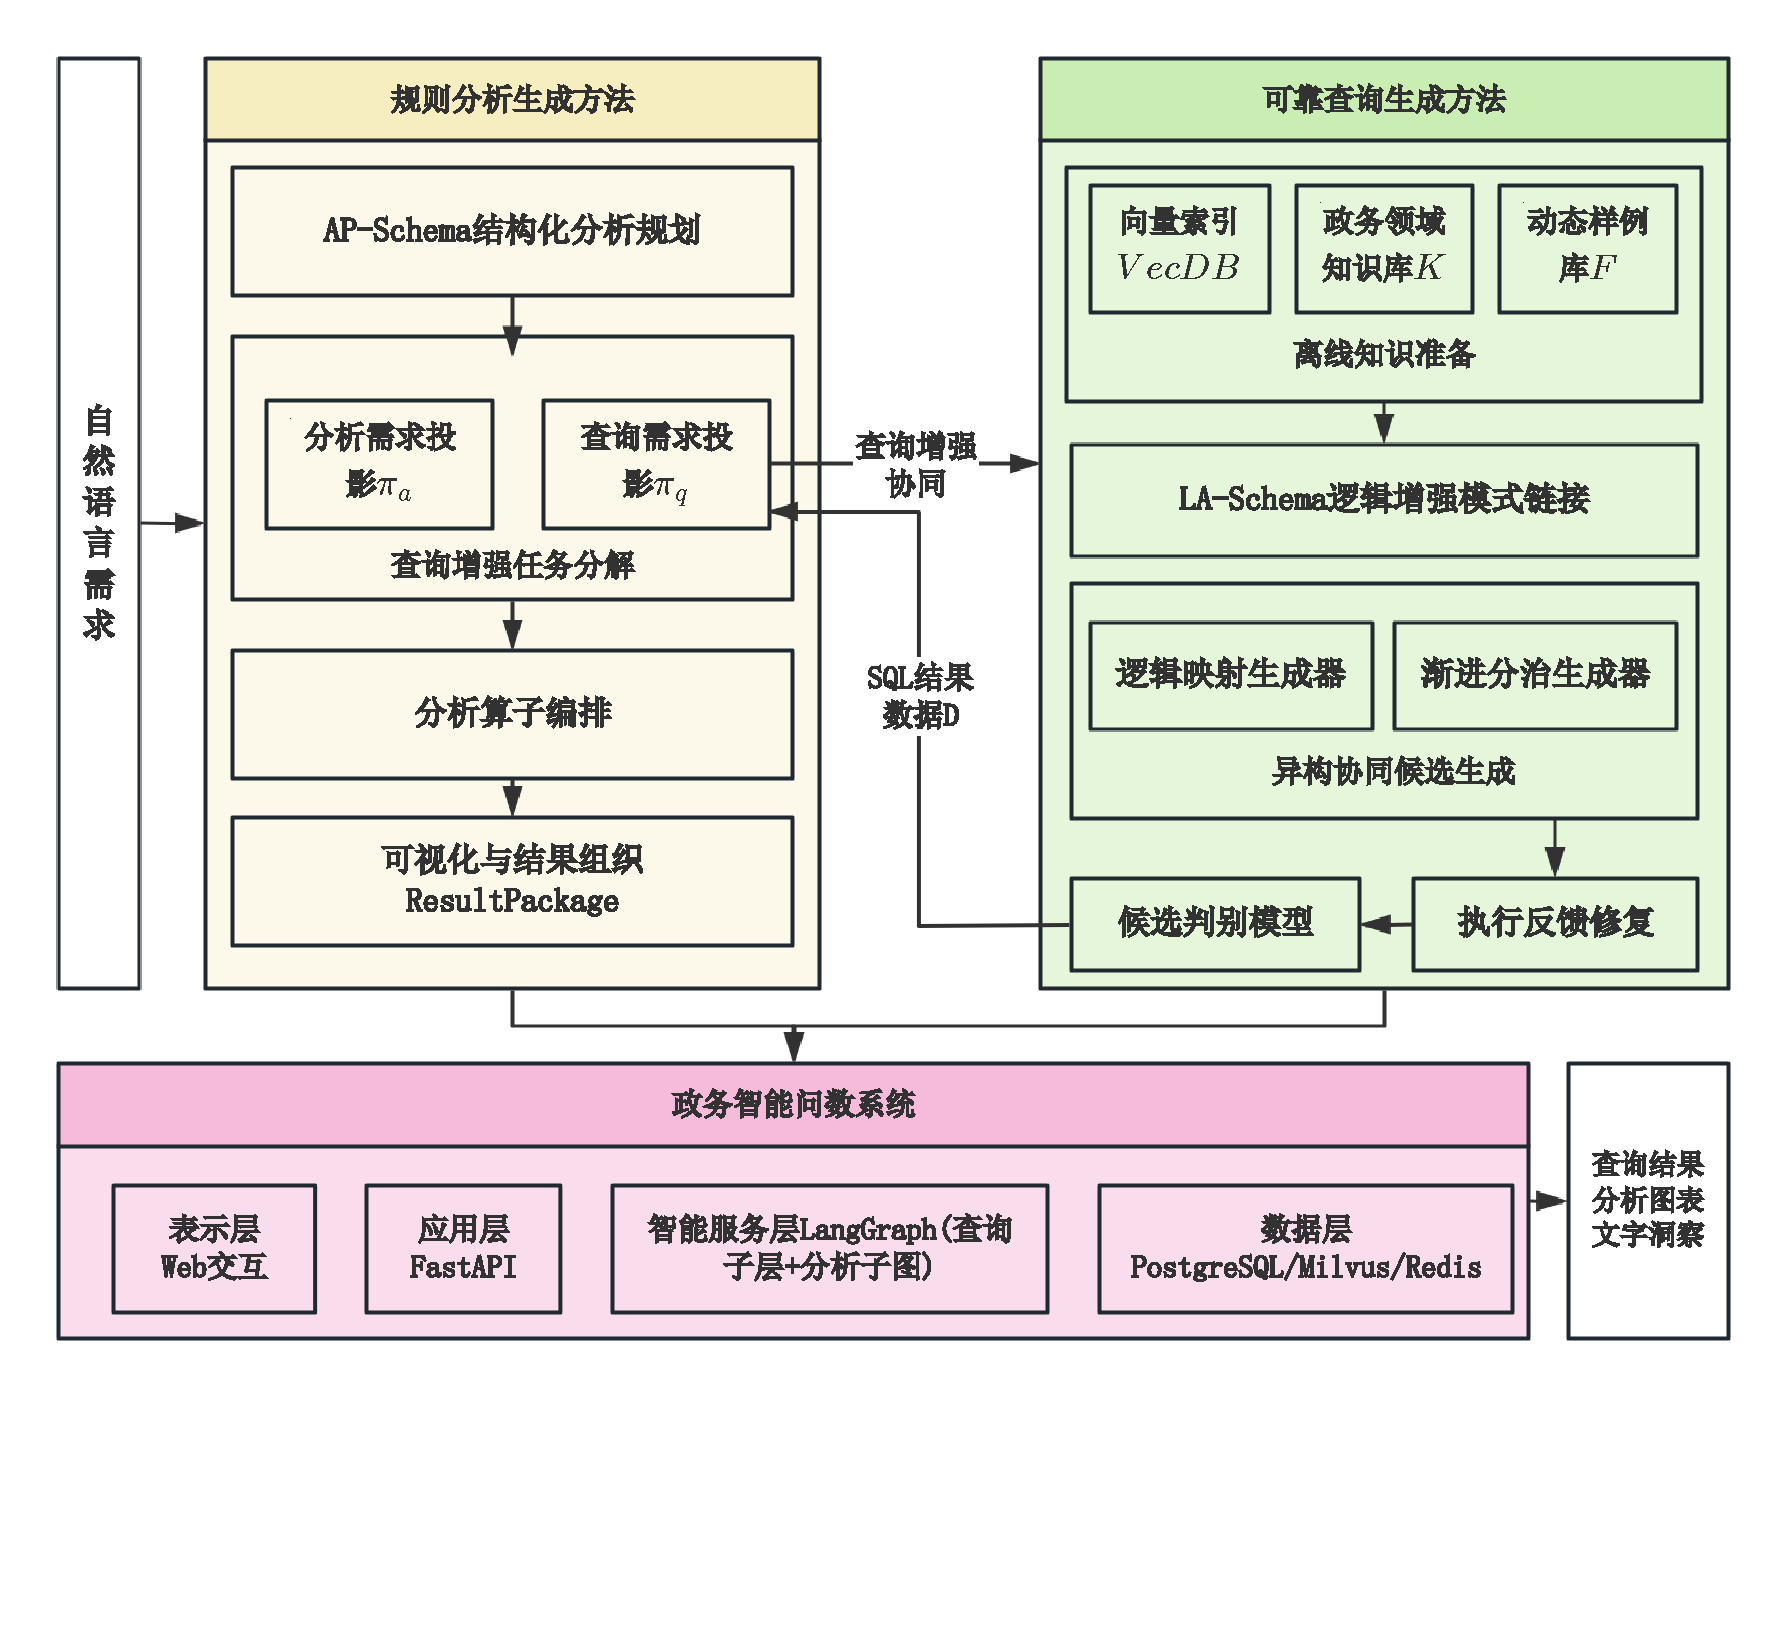
\includegraphics[width=0.85\textwidth]{figures/chap01/chap01-paper-chain.pdf}
	\caption{本文整体研究框架与技术链路示意图}
	\label{fig:chap01_research_framework}
\end{figure}

\textbf{（1）基于逻辑增强与异构协同的政务数据查询生成方法。}
针对政务数据查询中业务术语语义模糊、逻辑计算隐含和复杂查询结构长尾分布等问题，本文提出一种面向政务场景的Text-to-SQL方法。该方法在离线阶段构建向量索引数据库、政务领域知识库和动态样例库，在在线推理阶段设计逻辑增强模式LA-Schema，将业务术语映射、逻辑计算公式和值域约束显式注入数据库模式；同时设计逻辑映射生成器和渐进分治生成器组成的异构协同候选生成机制，并结合执行反馈驱动的查询修复和基于微调的候选判别模型，提高最终SQL查询的准确性、执行成功率与稳定性。该研究对应第三章，目标是解决政务场景下“查准”和“查稳”的问题。

\textbf{（2）基于分析规划与查询增强的政务数据分析方法。}
针对政务分析任务中需求约束复杂、查询与分析职责耦合以及结果表达需规范化等问题，本文提出一种协同查询能力的数据分析方法。该方法首先引入分析规划模式AP-Schema，将自然语言分析需求转化为包含分析类型、指标、维度、筛选条件、统计粒度、操作分层和可视化规格的结构化中间表示；其次，通过查询增强的任务分解机制，将涉及统计口径、模式理解和复杂关联的操作下沉至查询模块完成，而分析模块仅在可靠查询结果上执行排序、占比、透视、标注等轻量分析操作；最后结合分析算子库和可视化规则，生成图表、表格、文字洞察和日志组成的标准化结果包。该研究对应第四章，目标是解决政务场景下“怎么分析”和“如何规范输出”的问题。

\textbf{（3）政务智能问数系统设计与实现。}
在前述查询方法和分析方法基础上，本文进一步设计并实现一个面向政务场景的智能问数系统。系统采用表示层、应用层、智能服务层和数据层四层架构：应用层以FastAPI构建统一HTTP入口，支持同步查询与异步分析两类调用方式；智能服务层以LangGraph组织查询子图和分析子图，使分析流程通过AP-Schema投影查询约束后复用查询能力；数据层利用PostgreSQL保存系统元数据和领域知识，利用Milvus承载向量索引，利用Redis支持缓存和流式事件通道，实现结果产物、执行日志和会话状态的持久化管理。该研究对应第五章，目标是将方法创新转化为可交互、可追溯和可展示的系统能力。


\section{论文章节安排}

本文共分为六章，如图\ref{fig:chap01_paper-organize}.
各章内容安排如下。

\begin{figure}[htbp]
	\centering
	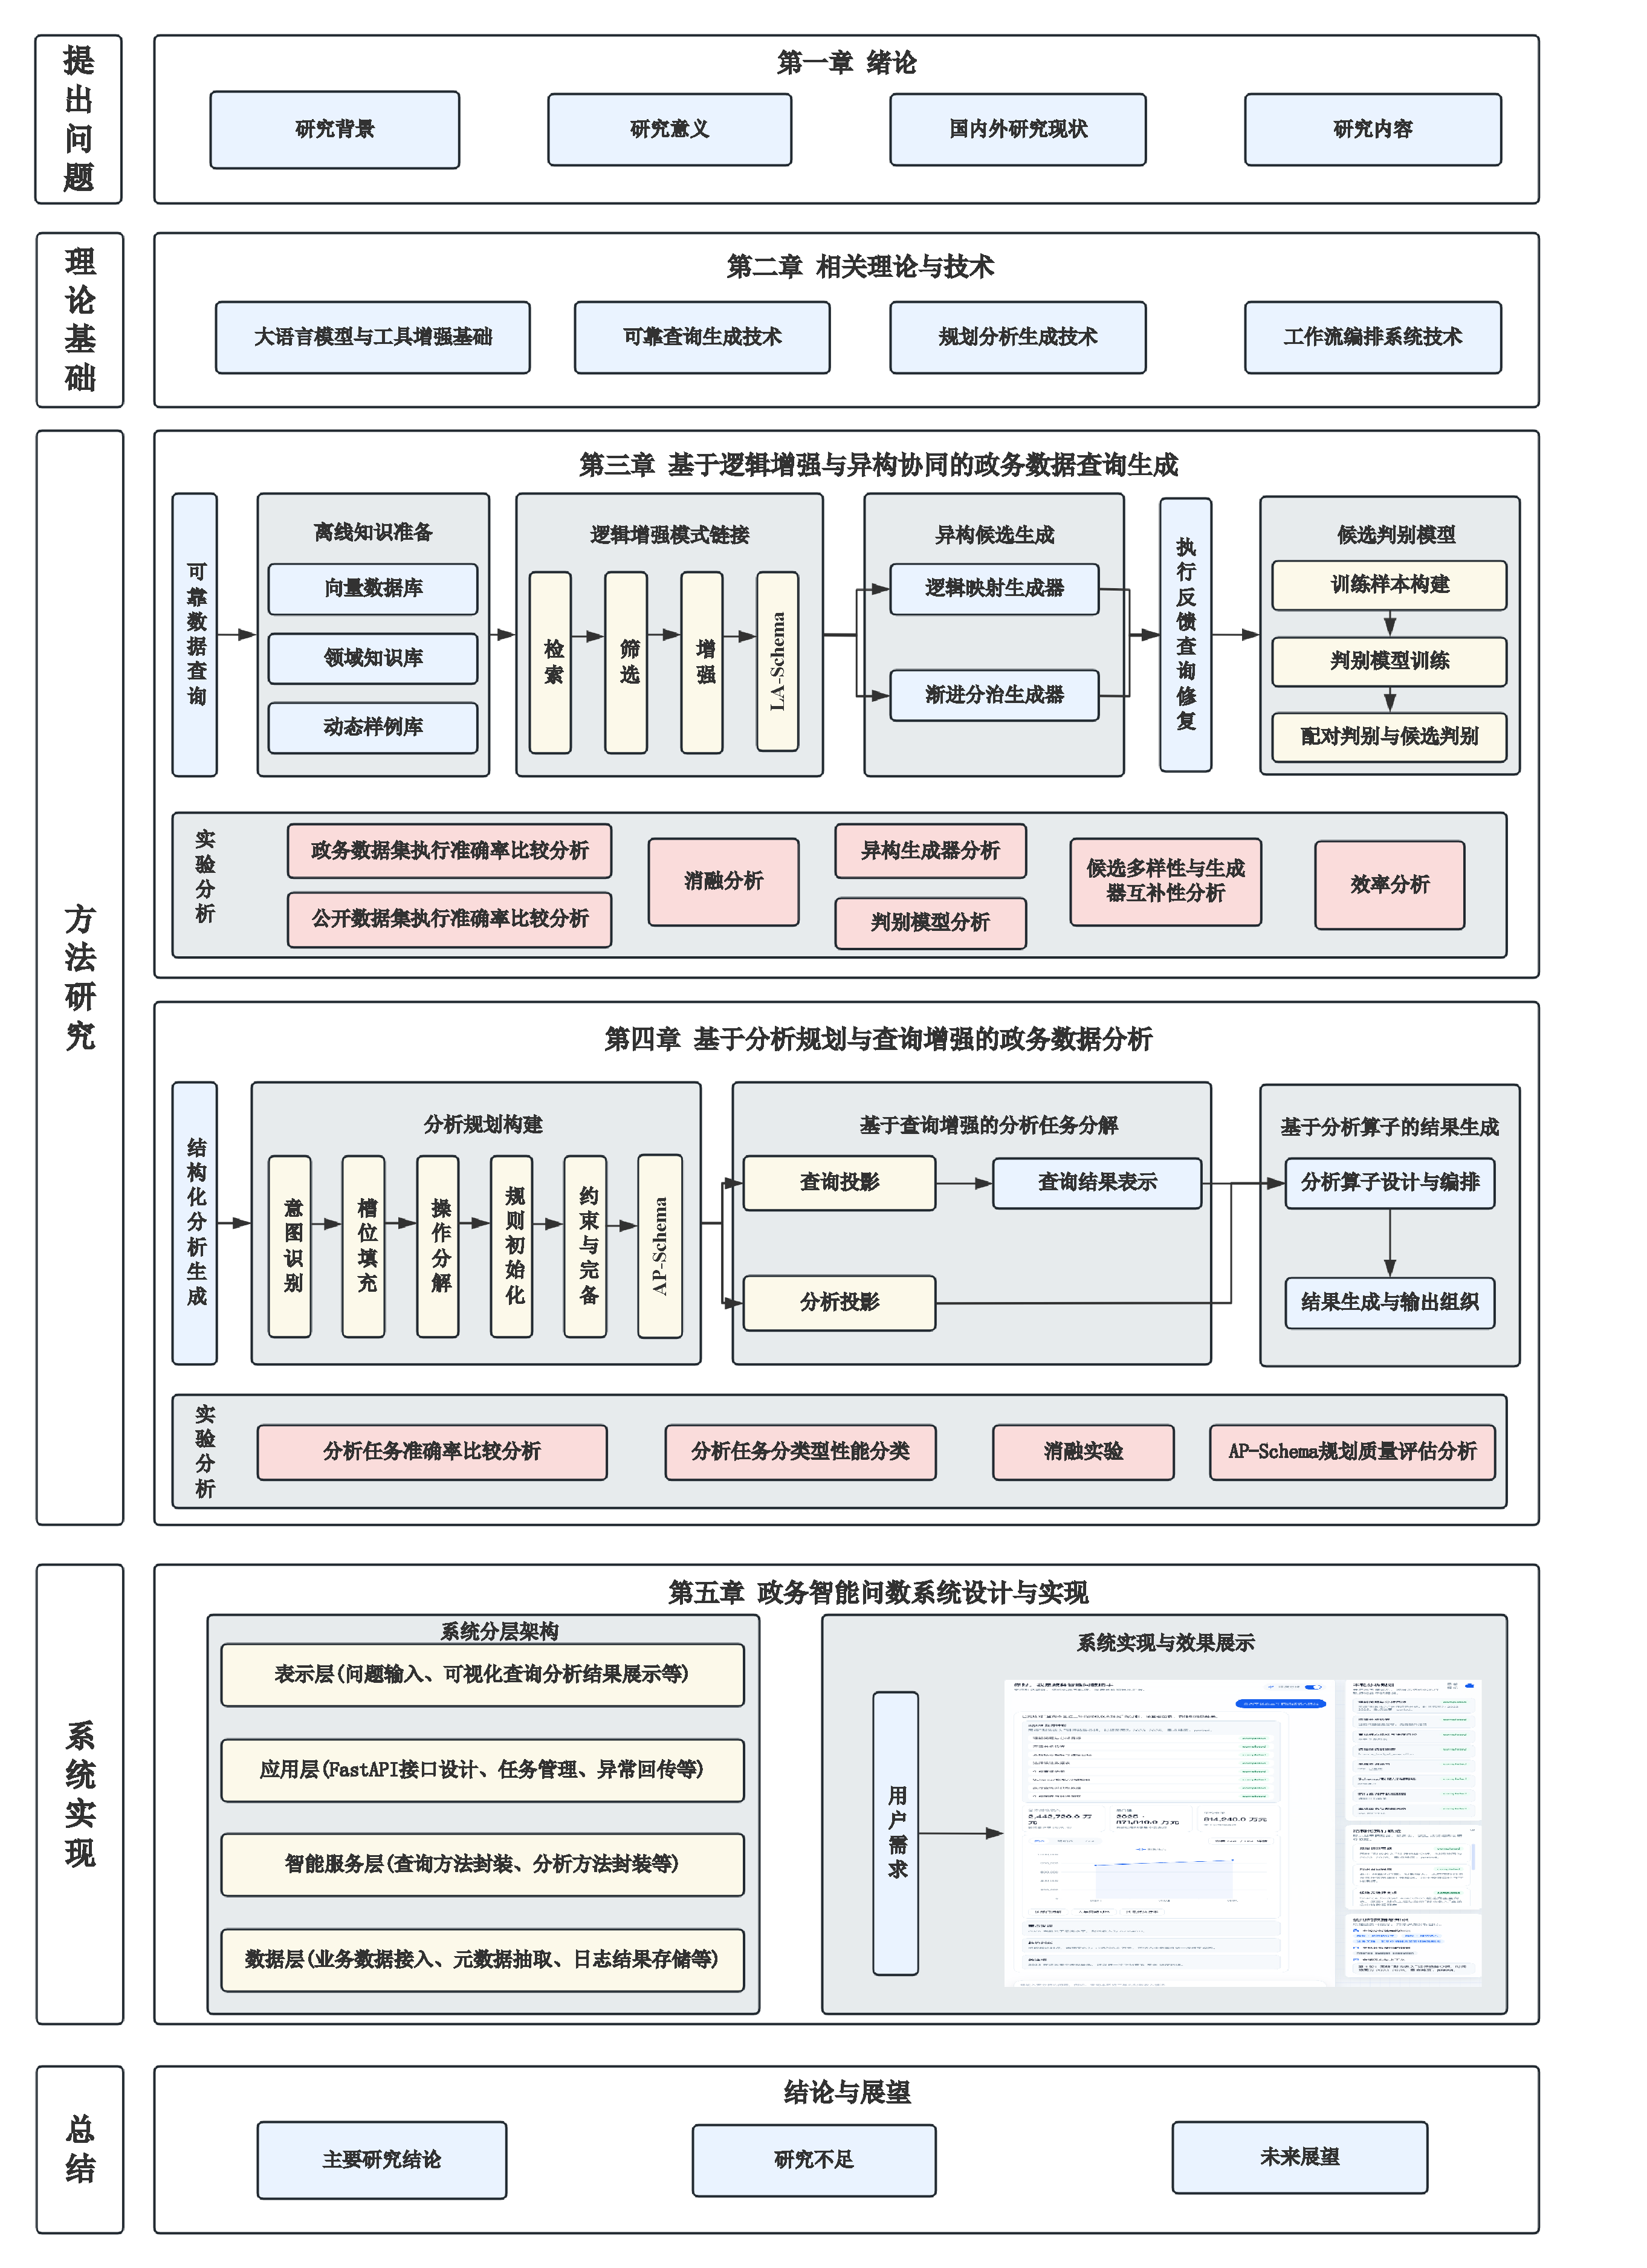
\includegraphics[width=0.85\textwidth]{figures/chap01/chap01-paper-organize.pdf}
	\caption{章节内容安排}\label{fig:chap01_paper-organize}
\end{figure}

\textbf{第一章，绪论。}
阐述论文的研究背景与意义，综述国内外相关研究现状，归纳当前存在的关键问题，并给出本文的研究内容与整体结构安排。

\textbf{第二章，相关理论与技术。}
介绍论文所依赖的理论基础与关键技术，包括大语言模型与工具增强基础、面向可靠查询生成的关键技术、面向数据分析的规划与结果生成技术，以及面向系统实现的工作流编排与服务协同技术。

\textbf{第三章，基于逻辑增强与异构协同的政务数据查询生成方法。}
围绕政务场景中的可靠取数问题，提出包含离线知识准备、逻辑增强模式链接、异构候选生成、执行反馈修复和候选判别选择在内的Text-to-SQL方法，并通过自建政务数据集和公共数据集实验验证方法有效性。

\textbf{第四章，基于分析规划与查询增强的政务数据分析方法。}
围绕政务场景中的结构化分析问题，提出AP-Schema分析规划模式、查询增强的任务分解机制、分析算子编排与标准化结果组织方法，并通过多维实验验证其性能与规划质量。

\textbf{第五章，政务智能问数系统设计与实现。}
在前两章方法基础上，设计并实现一个政务智能问数系统，介绍系统总体架构、应用层与智能服务层实现、系统数据层存储以及系统功能展示与效果。

\textbf{第六章，结论与展望。}
总结全文研究工作与主要创新点，分析现有工作的不足，并对后续研究方向进行展望。


\section{本章小结}

本章围绕数字政府建设和政务数据资源利用的现实需求，阐明了本文开展政务智能问数研究的背景、目标与意义；在系统梳理Text-to-SQL、自动数据分析以及政务数据管理与应用平台相关研究进展的基础上，归纳出领域知识显式增强不足、分析规划与查询协同不足、系统化落地能力不足三个关键问题，并说明了开展本研究既具有现实必要性，也具备明确技术可行性；进而明确了本文围绕政务数据查询生成方法、政务数据分析方法和智能问数系统实现展开研究的总体思路，并说明了全文的章节安排，为后续章节展开奠定基础。
